\subsection{Universidad de Helsinki}

Resultados obtenidos en el monitoreo:\\

\smallskip
\begin{tabular}{| l | c | c | c | c |}
\hline
Hop & IP &  RTT promedio (s)  & deltaRTT promedio & Ubicacion\\ 
\hline
1 & 192.168.11.1 & 0.01142361429 & 0.01142361429 & Argentina, Buenos Aires\\
\hline
2 & 10.21.128.1 & 0.0283621417152 & 0.0169385274251 & Argentina, Buenos Aires\\
\hline
3 & 10.242.0.201 & 0.0378749105665 & 0.00951276885139 & Argentina, Buenos Aires\\
\hline
4 & 195.22.220.33 & 0.0143795543247 & 0 & Italy\\
\hline
5 & 195.22.220.32 & 0.292960882187 & 0.278581327862 & Italy\\
\hline
6 & 89.221.41.171 & 0.152727180057 & 0 & Italy\\
\hline
7 & 89.221.41.171 & 0.156960460875 & 0.00423328081767 & Italy\\
\hline
8 & 154.54.9.17 & 0.202791770299 & 0.0458313094245 & United States\\
\hline
9 & 154.54.80.41 & 0.21254154614 & 0.00974977584112 & United States\\
\hline
10 & 66.28.4.237 & 0.168935351902 & 0 & United States, Pasadena\\
\hline
11 & 154.54.29.222 & 0.251122385263 & 0.0821870333619 & United States\\
\hline
12 & 154.54.42.77 & 0.316137870153 & 0.0650154848893 & United States\\
\hline
13 & 154.54.45.162 & 0.327892038557 & 0.0117541684045 & United States\\
\hline
14 & 154.54.45.2 & 0.255609459347 & 0 & United States\\
\hline
15 & 38.88.196.186 & 0.270633061727 & 0.0150236023797 & United States, Los Angeles\\
\hline
16 & 101.4.117.169 & 0.435372935401 & 0.164739873674 & China, Beijing\\
\hline
17 & 101.4.117.97 & 0.467933893204 & 0.0325609578027 & China, Beijing\\
\hline
18 & 101.4.112.105 & 0.437322590086 & 0 & China, Beijing\\
\hline
19 & 101.4.118.94 & 0.43985332383 & 0.0025307337443 & China, Beijing\\
\hline
20 & 101.4.112.90 & 0.435603486167 & 0 & China, Beijing\\
\hline
21 & 101.4.117.81 & 0.413042836719 & 0 & China, Beijing\\
\hline
22 & 202.112.41.178 & 0.405184189479 & 0 & China, Shanghai\\
\hline
23 & 202.112.41.182 & 0.394645796882 & 0 & China, Shanghai\\
\hline
24 & 162.105.252.133 & 0.488684309853 & 0.0940385129717 & China, Beijing\\
\hline
\end{tabular}
\bigskip

\textbf{Paquetes enviados: 407 / Paquetes no respondidos: 37}\\

\textbf{Tres outliers, hops: 4, 6 y 8}\\

[INSERTE ANÁLISIS AQUÍ]

A continuación mostramos un gráfico con los RTT entre saltos y otro con los ZRTT\footnote{ZRTT = $(X_i - \bar{X}) / S$}  entre saltos. También así el planisferio con los saltos graficados.

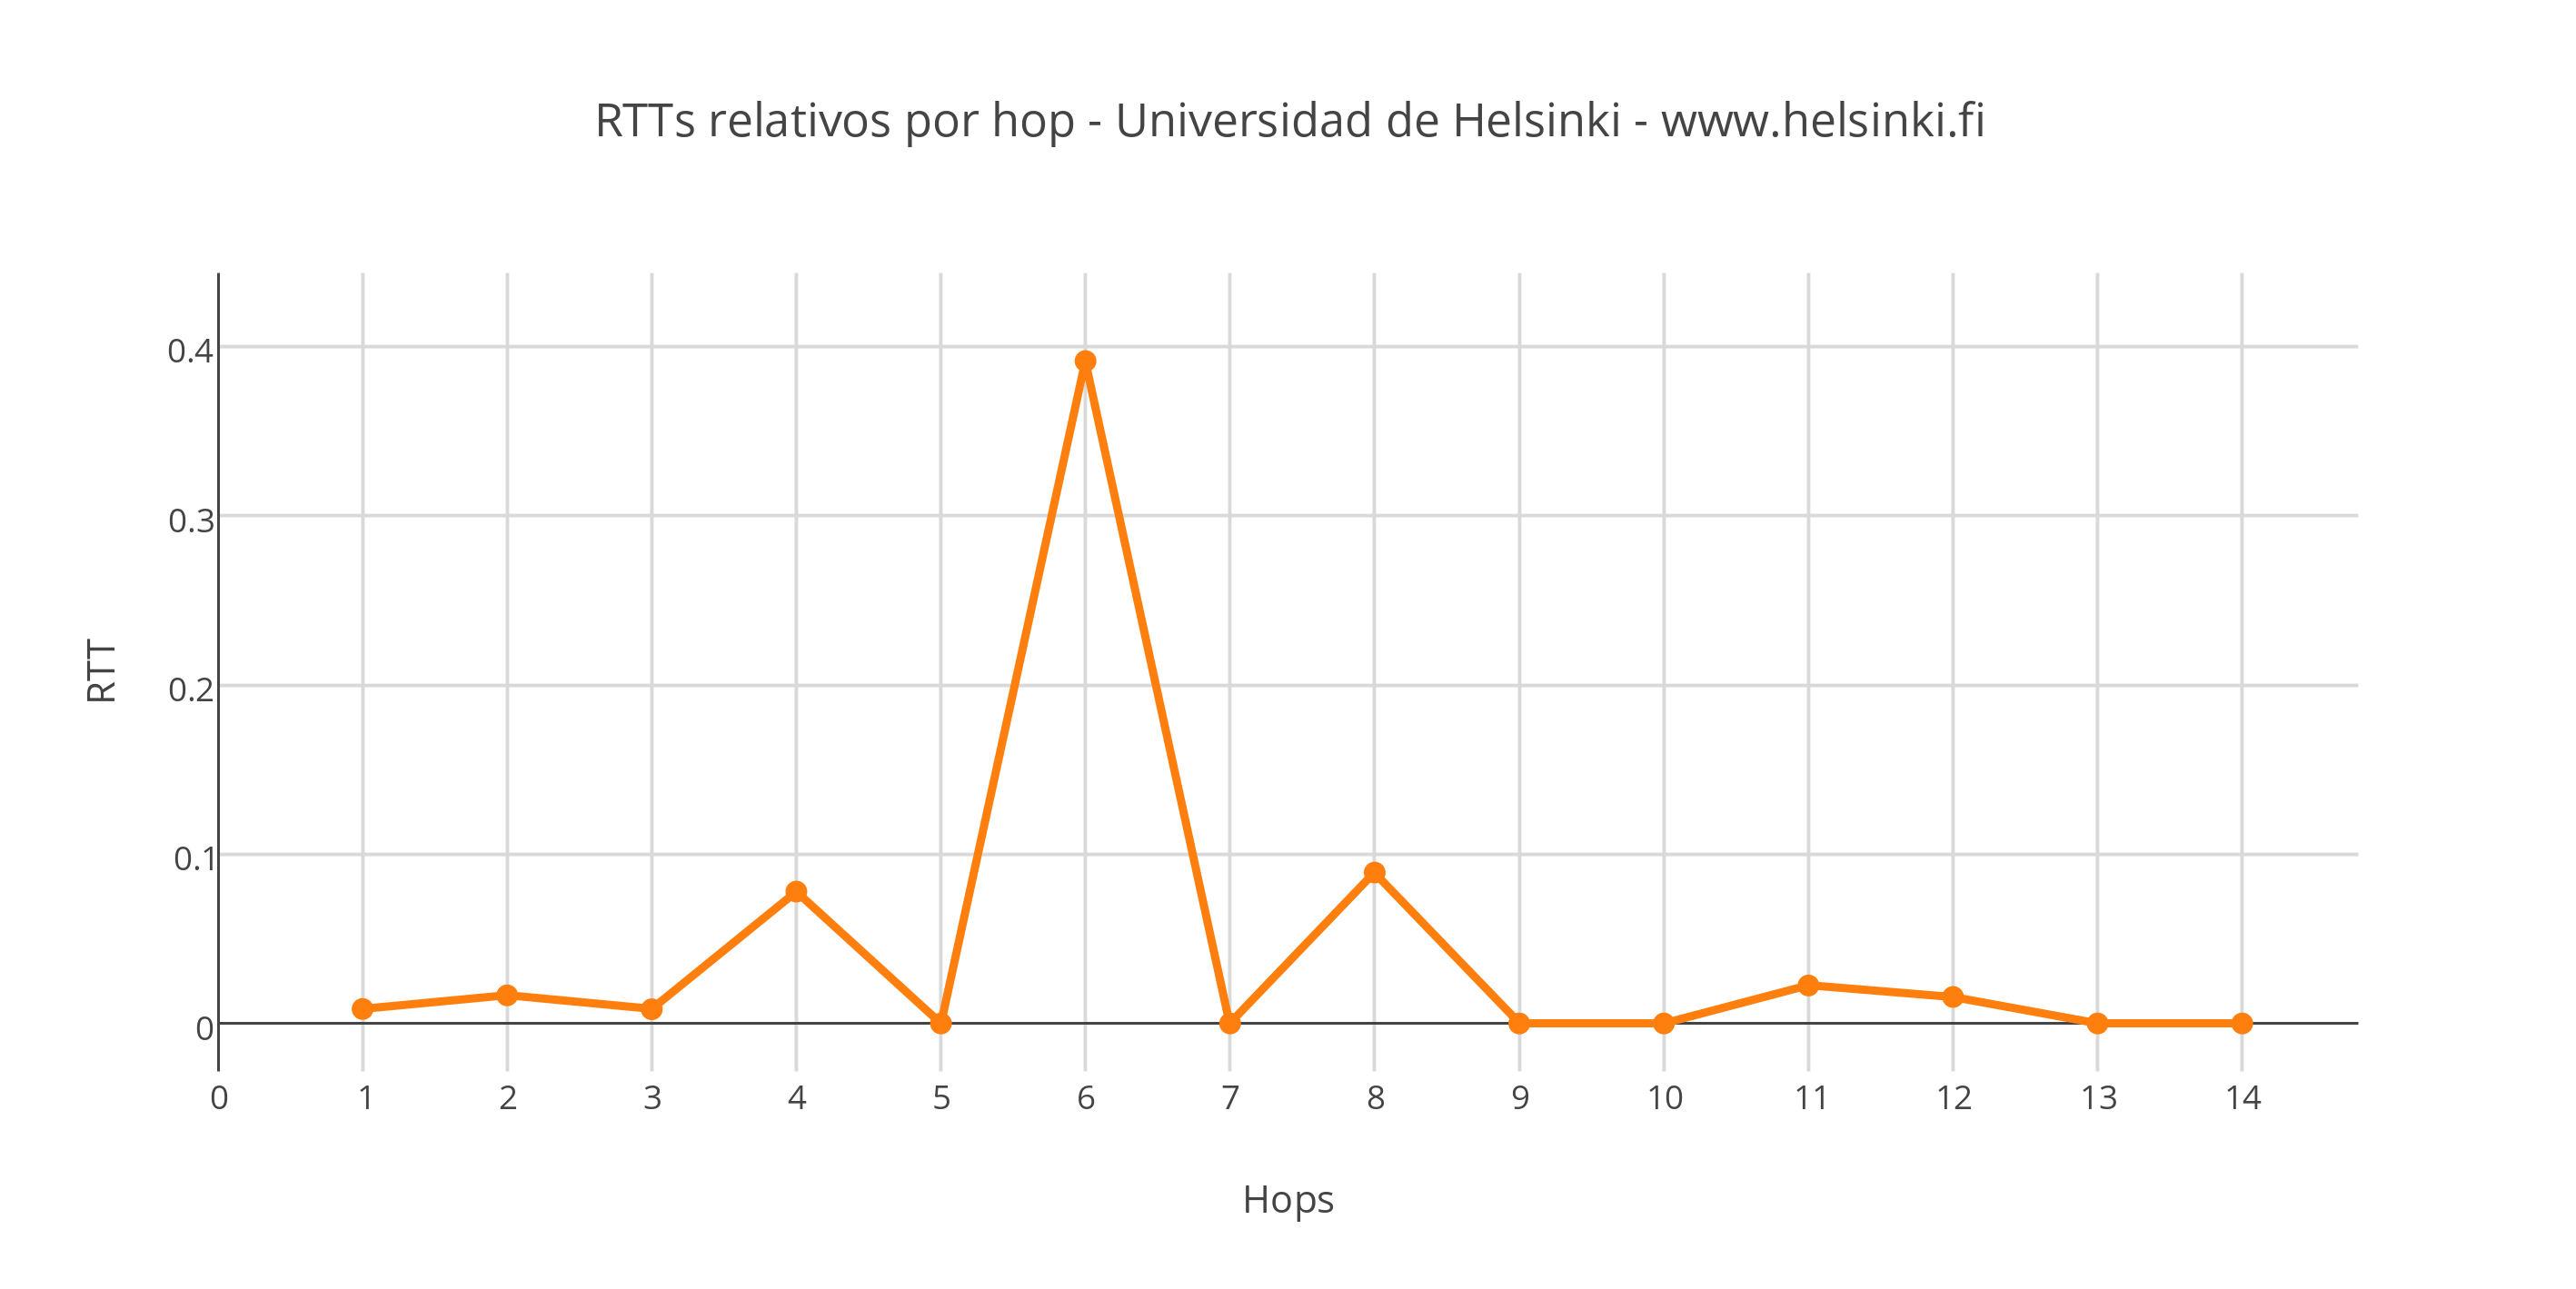
\includegraphics[scale=0.65]{imagenes/helsinki/RTTs.png} 

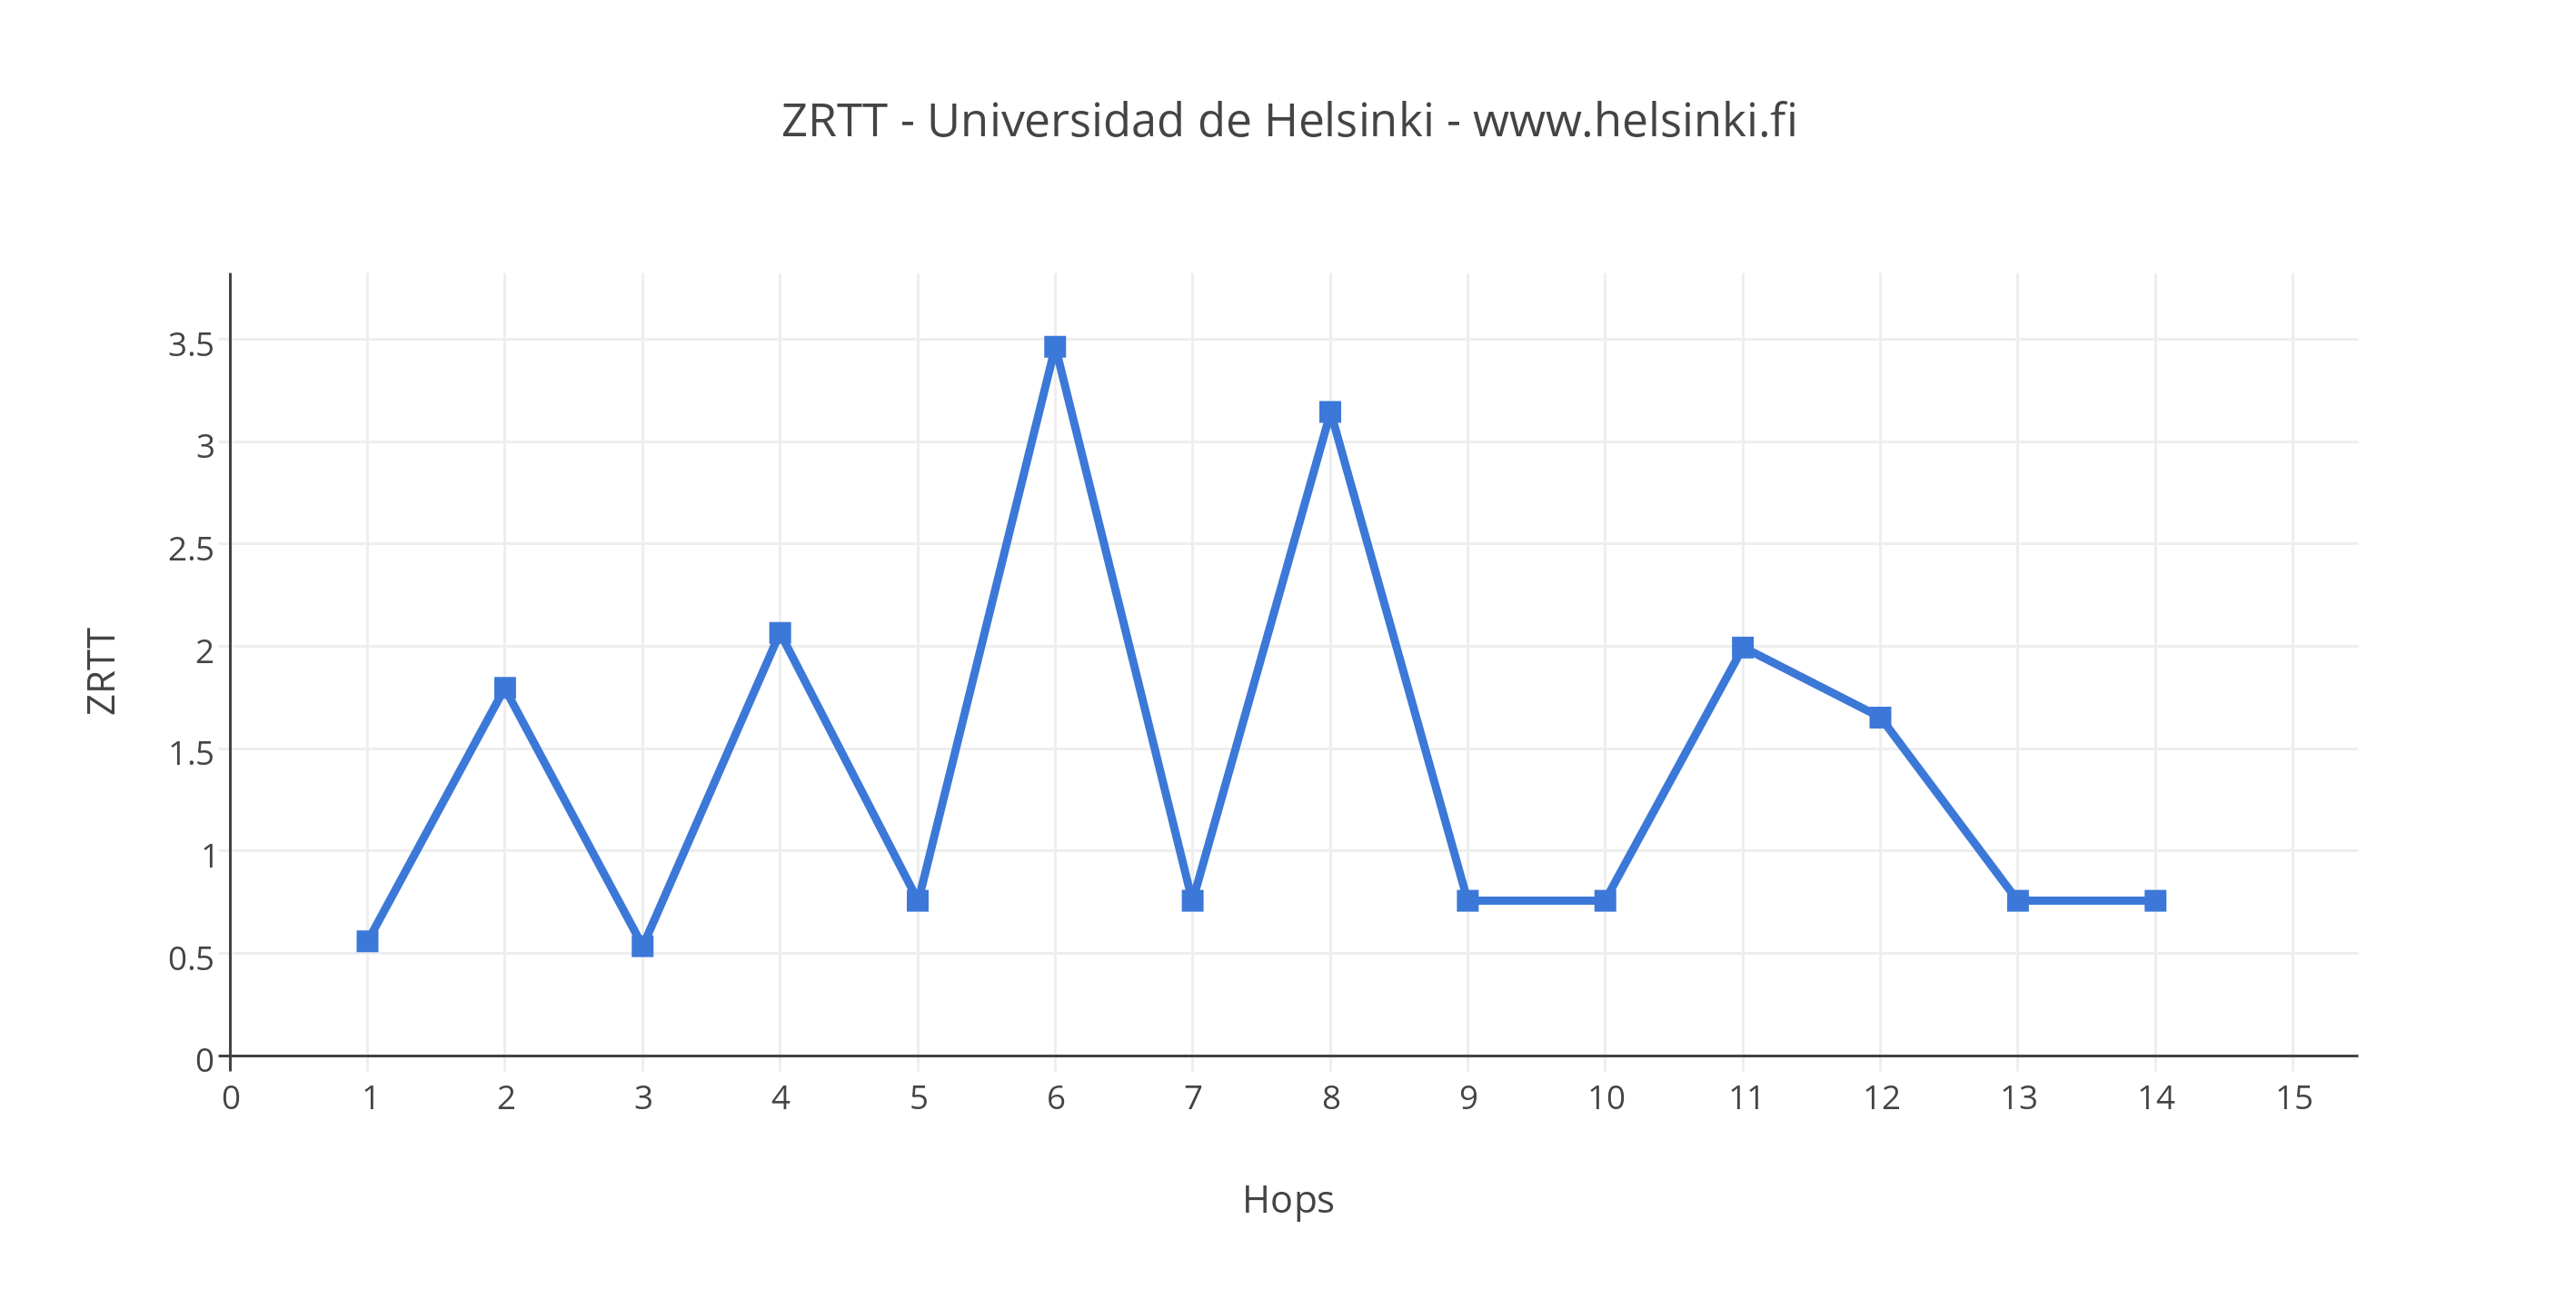
\includegraphics[scale=0.65]{imagenes/helsinki/ZRTTs.png} 

\begin{center}
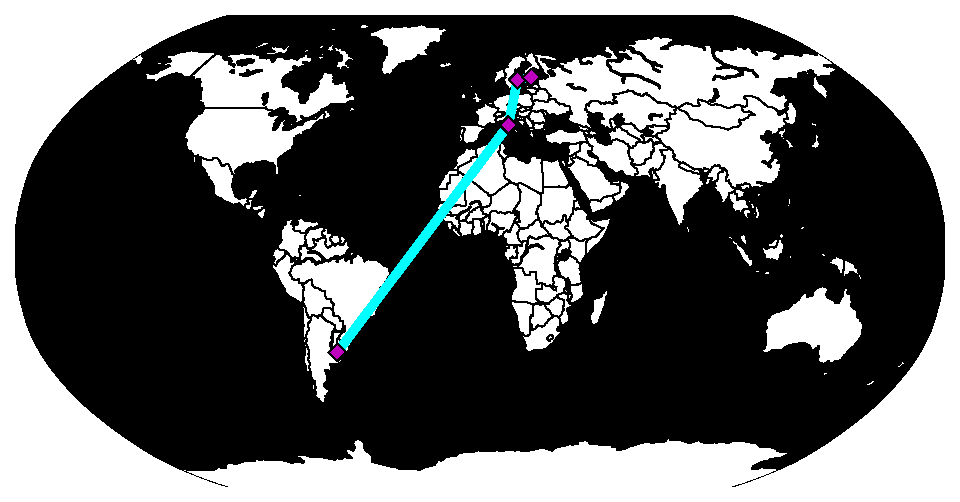
\includegraphics[scale=0.8]{imagenes/helsinki/helsinki.pdf} 
\end{center}